\documentclass{article}
\usepackage[
  a4paper,
  left=2cm, right=2cm,
  top=2cm, bottom=2cm
]{geometry}
\usepackage{graphicx} % Required for inserting images
\usepackage{amsmath}       % Équations avancées
\usepackage{amssymb}       % Symboles mathématiques
\usepackage{graphicx}      % Inclusion de figures
\usepackage{siunitx}       % Unités SI
\usepackage{setspace}
\singlespacing
\usepackage{multirow}
\usepackage{booktabs}      % Tableaux professionnels
\usepackage[table]{xcolor}
\usepackage{hyperref}      % Références cliquables
\usepackage[most]{tcolorbox}
\usepackage{bm}
\usepackage{verbatim}

\usepackage[framemethod=TikZ]{mdframed}
\usepackage{pgfplots}   
\usepackage{caption}   

\usepackage{enumitem}
\usepackage{titlesec}
\usepackage{wasysym}
\usepackage{tikz}
\usetikzlibrary{positioning,arrows.meta,shapes.geometric,decorations.pathreplacing,calc,3d,positioning,patterns} % pour "below=of ..." et "-Stealth"
\usepackage{tikz-3dplot}

\usepackage{algorithm}
\usepackage{algorithmic}

\usepackage{listings}
\usetikzlibrary{shapes,arrows,positioning,calc}

\usepackage{fancyvrb}
\usepackage{fvextra}
\usepackage{pifont}

\newcommand{\codeTight}{\fontsize{8pt}{9pt}\selectfont} 

\captionsetup{font=footnotesize,labelfont=bf,textfont=it,skip=0pt}

% Commandes personnalisées
\newcommand{\cmark}{\textcolor{successgreen}{\ding{51}}}
\newcommand{\xmark}{\textcolor{errorred}{\ding{55}}}
\newcommand{\wmark}{\textcolor{warningorange}{\ding{45}}}


% --- Espaces autour des flottants (tables, figures) ---
\setlength{\textfloatsep}{8pt plus 2pt minus 2pt}
\setlength{\floatsep}{8pt plus 2pt minus 2pt}
\setlength{\intextsep}{8pt plus 2pt minus 2pt}
\setlength{\abovecaptionskip}{4pt}
\setlength{\belowcaptionskip}{0pt}

% --- Listes pour tout le document ---
\setlist[itemize]{itemsep=0pt, topsep=2pt, parsep=0pt, partopsep=0pt}
\setlist[enumerate]{itemsep=0pt, topsep=2pt, parsep=0pt, partopsep=0pt}

% --- Espaces autour des titres ---
\titlespacing*{\section}
  {0pt}{2ex plus 1ex minus .2ex}{1ex plus .5ex minus .2ex}
\titlespacing*{\subsection}
  {0pt}{1.5ex plus .5ex minus .2ex}{0.7ex plus .3ex minus .1ex}

% --- Espaces autour des formules affichées ---
\setlength{\abovedisplayskip}{6pt}
\setlength{\belowdisplayskip}{6pt}
\setlength{\abovedisplayshortskip}{4pt}
\setlength{\belowdisplayshortskip}{4pt}

\definecolor{misty}{rgb}{1.0,0.89,0.88}
\definecolor{MyBlue}{rgb}{0.8,1.0,1.0}
\definecolor{Carnelian}{rgb}{0.7,0.11,0.11}
\definecolor{MyGreen}{rgb}{0.0,0.5,0.0}
\definecolor{MyGreen2}{rgb}{0.0,0.42,0.24}
\definecolor{corrigecolor}{RGB}{180,100,200}
\definecolor{methode1color}{RGB}{220,80,60}
\definecolor{methode2color}{RGB}{80,180,80}
\definecolor{lightblue}{RGB}{220,235,255}
\definecolor{successgreen}{RGB}{39,174,96}
\definecolor{warningorange}{RGB}{243,156,18}
\definecolor{errorred}{RGB}{231,76,60}
\definecolor{infoblue}{RGB}{52,152,219}
\definecolor{darkblue}{RGB}{44,62,80}
\definecolor{lightgray}{RGB}{245,245,245}
\definecolor{purple}{RGB}{142,68,173}

% Définition des couleurs
\definecolor{source}{RGB}{255,50,50}
\definecolor{cone60}{RGB}{255,200,100}
\definecolor{coneplaque}{RGB}{0,180,0}
\definecolor{conedetecteur}{RGB}{0,100,200}
\definecolor{wpetg}{RGB}{0,150,0}
\definecolor{water}{RGB}{0,100,200}


% Configuration des couleurs
\definecolor{typeA}{RGB}{231,76,60}
\definecolor{typeB}{RGB}{241,196,15}
\definecolor{typeC}{RGB}{230,126,34}
\definecolor{typeD0}{RGB}{155,89,182}
\definecolor{typeD1}{RGB}{52,152,219}
\definecolor{typeD2}{RGB}{26,188,156}
\definecolor{typeD3}{RGB}{46,204,113}
\definecolor{typeD4}{RGB}{149,165,166}

\definecolor{methode1}{RGB}{70,130,180}
\definecolor{methode1bis}{RGB}{60,179,113}
\definecolor{methode2}{RGB}{255,140,0}
\definecolor{theoriecolor}{RGB}{0,100,180}

% Couleurs
\definecolor{darkblue}{RGB}{0,51,102}
\definecolor{lightblue}{RGB}{230,240,250}
\definecolor{lightgreen}{RGB}{230,250,230}
\definecolor{lightorange}{RGB}{255,240,220}
\definecolor{lightred}{RGB}{255,230,230}
\definecolor{method1}{RGB}{70,130,180}
\definecolor{method1bis}{RGB}{60,179,113}
\definecolor{method2}{RGB}{255,140,0}


% Couleurs personnalisées
\definecolor{sourcecolor}{RGB}{255,100,0}
\definecolor{matrixcolor}{RGB}{255,220,100}
\definecolor{upstreamcolor}{RGB}{100,100,255}
\definecolor{downstreamcolor}{RGB}{255,100,100}
\definecolor{watercolor}{RGB}{100,180,255}
\definecolor{conecolor}{RGB}{255,200,100}
\definecolor{aircolor}{RGB}{240,248,255}
\definecolor{warningcolor}{RGB}{255,150,0}
\definecolor{energie40}{RGB}{255,100,100}
\definecolor{energie122}{RGB}{255,150,50}
\definecolor{energie344}{RGB}{255,200,50}
\definecolor{energie779}{RGB}{150,200,50}
\definecolor{energie964}{RGB}{50,200,100}
\definecolor{energie1408}{RGB}{50,150,200}

% Couleurs personnalisées
\definecolor{airblue}{RGB}{135,206,250}
\definecolor{sourcemagenta}{RGB}{255,0,255}
\definecolor{conecolor}{RGB}{255,200,0}
\definecolor{kermacolor}{RGB}{0,255,255}
\definecolor{upstreamblue}{RGB}{0,0,255}
\definecolor{downstreamred}{RGB}{255,0,0}
\definecolor{slabcolor}{RGB}{255,255,0}
\definecolor{plaquecolor}{RGB}{100,200,100}
\definecolor{cone60color}{RGB}{100,200,100}
\definecolor{cone7color}{RGB}{255,150,150}

% Couleurs personnalisées
\definecolor{wpetg}{RGB}{0,150,0}
\definecolor{bismuth}{RGB}{180,100,180}
\definecolor{petg}{RGB}{100,150,200}
\definecolor{air}{RGB}{200,220,255}
\definecolor{water}{RGB}{0,100,200}
\definecolor{source}{RGB}{255,50,50}
\definecolor{cone}{RGB}{255,200,100}

% Couleurs personnalisées
\definecolor{sourcecolor}{RGB}{255,100,100}
\definecolor{slabcolor}{RGB}{255,230,100}
\definecolor{upstreamcolor}{RGB}{100,150,255}
\definecolor{downstreamcolor}{RGB}{255,100,100}
\definecolor{kermacolor}{RGB}{100,255,255}
\definecolor{aircolor}{RGB}{220,240,255}
\definecolor{conecolor}{RGB}{255,200,150}
\definecolor{worldcolor}{RGB}{240,240,240}
\definecolor{envelopecolor}{RGB}{200,220,255}

\definecolor{transmitcolor}{RGB}{46,204,113}
\definecolor{absorbcolor}{RGB}{231,76,60}
\definecolor{scattercolor}{RGB}{241,196,15}
\definecolor{oldcolor}{RGB}{180,180,180}

% Couleurs personnalisées
\definecolor{aircolor}{RGB}{200,230,255}
\definecolor{watercolor}{RGB}{100,150,255}
\definecolor{sourcecolor}{RGB}{255,80,80}
\definecolor{detectorcolor}{RGB}{100,200,100}
\definecolor{conecolor}{RGB}{255,180,100}
\definecolor{cone7color}{RGB}{100,200,255}
\definecolor{envelopecolor}{RGB}{230,230,230}
\definecolor{upstreamcolor}{RGB}{80,80,255}
\definecolor{downstreamcolor}{RGB}{255,80,80}
\definecolor{gammacolor}{RGB}{255,200,0}

% Couleurs
\definecolor{spherecolor}{RGB}{100,150,255}
\definecolor{raycolor}{RGB}{255,100,100}
\definecolor{chordcolor}{RGB}{50,200,50}
\definecolor{centercolor}{RGB}{0,0,0}
\definecolor{pointcolor}{RGB}{200,50,50}

\definecolor{wpetg}{RGB}{34,139,34}      % Vert forêt pour W/PETG
\definecolor{inox}{RGB}{192,192,192}     % Gris argent pour Inox
\definecolor{water}{RGB}{100,149,237}    % Bleu pour eau
\definecolor{source}{RGB}{255,215,0}     % Or pour source
\definecolor{gamma}{RGB}{255,69,0}       % Orange-rouge pour gammas

% Couleurs
\definecolor{lightgreen}{RGB}{220,255,220}
\definecolor{lightyellow}{RGB}{255,255,220}
\definecolor{lightblue}{RGB}{220,235,255}
\definecolor{bismuth}{RGB}{180,140,200}
\definecolor{petg}{RGB}{200,200,220}
\definecolor{eau}{RGB}{150,200,255}
\definecolor{air}{RGB}{240,248,255}
\definecolor{cone60}{RGB}{255,200,150}

% Boîtes colorées
\newtcolorbox{databox}[1]{
    colback=blue!5,
    colframe=blue!75!black,
    fonttitle=\bfseries,
    title=#1
}

\newtcolorbox{resultbox}[1]{
    colback=green!5,
    colframe=green!75!black,
    fonttitle=\bfseries,
    title=#1
}

\newtcolorbox{warningbox}[1]{
    colback=orange!5,
    colframe=orange!75!black,
    fonttitle=\bfseries,
    title=#1
}

% --- Espaces autour des flottants (tables, figures) ---
\setlength{\textfloatsep}{8pt plus 2pt minus 2pt}
\setlength{\floatsep}{8pt plus 2pt minus 2pt}
\setlength{\intextsep}{8pt plus 2pt minus 2pt}
\setlength{\abovecaptionskip}{4pt}
\setlength{\belowcaptionskip}{0pt}

% --- Listes pour tout le document ---
\setlist[itemize]{itemsep=0pt, topsep=2pt, parsep=0pt, partopsep=0pt}
\setlist[enumerate]{itemsep=0pt, topsep=2pt, parsep=0pt, partopsep=0pt}

% --- Espaces autour des titres ---
\titlespacing*{\section}
  {0pt}{2ex plus 1ex minus .2ex}{1ex plus .5ex minus .2ex}
\titlespacing*{\subsection}
  {0pt}{1.5ex plus .5ex minus .2ex}{0.7ex plus .3ex minus .1ex}

% --- Espaces autour des formules affichées ---
\setlength{\abovedisplayskip}{6pt}
\setlength{\belowdisplayskip}{6pt}
\setlength{\abovedisplayshortskip}{4pt}
\setlength{\belowdisplayshortskip}{4pt}

\title{
\vspace{-1cm}
{\color{blue}\rule{\linewidth}{2pt}}\\[0.5cm]
{\Huge\bfseries Simulation Monte Carlo Geant4}\\[0.3cm]
{\Large Effet d'une Plaque W/PETG sur le Débit de Dose}\\[0.3cm]
{\large Source Eur152 - Cône 60° -25 Millions d'Événements}\\[0.3cm]
{\color{Carnelian}\rule{\linewidth}{2pt}}
}
\title{\textbf{Analyse des Méthodes de Calcul du dose\\dans une Simulation Geant4}\\[0.5cm]
\large Source Europium-152 -- Détecteur dans l'air à 20 cm -- plaque intermédiaire pleine W/PETG (18mm)}
\author{Documentation technique}
\date{\today}

\begin{document}

\maketitle

\begin{abstract}
Ce document présente une analyse comparative de méthodes de calcul grandeurs radiométriques (débit de Kerma, débit de dose dans des tissus mous),  implémentées dans la simulation Geant4 d'une source d'Europium-152.\newline La première méthode repose sur le dépôt d'énergie Monte Carlo, tandis que la seconde utilise le calcul par fluence avec les coefficients d'absorption d'énergie tabulés. Cette analyse inclut les fondements théoriques, l'implémentation informatique et les conditions de validité de chaque approche.
\end{abstract}

\newpage

\tableofcontents

\newpage

%==============================================================================
\normalsize
\noindent \begin{mdframed}[backgroundcolor=orange!20]
\section{\Large \color{blue} \textbf{Configuration de la simulation}\color{black}}
\end{mdframed}
\footnotesize
%==============================================================================

\begin{tcolorbox}[colback=blue!5,colframe=blue,title=\textbf{Nouvelle Configuration}]
\noindent ${\rm \; \; \; \; \; \; \; \;}$ \; \textbf{-} \; la \color{blue}\textbf{plaque intermediaire}\color{black} \; a une épaisseur de 18 mm\newline
\noindent ${\rm \; \; \; \; \; \; \; \;}$ \; \textbf{-} \; la \color{blue}\textbf{plaque intermediaire}\color{black} \; est un bloc de \textbf{W/PETG} de 100 $\times$ 100 $\times$ 18 mm\newline
\noindent ${\rm \; \; \; \; \; \; \; \;}$ \; \textbf{-} \; Son centre est en $\bm{z}$ = 4.65 cm (2.65 cm de la source)\newline
\noindent ${\rm \; \; \; \; \; \; \; \;}$ \; \textbf{-} \;  Les plans de comptage sont distant de $\bm{z}$ = 2mm des faces avants et arriéres de la plaque\newline
\noindent ${\rm \; \; \; \; \; \; \; \;}$ \; \textbf{-} \; Le centre du \color{blue}\textbf{détecteur sphèrique}\color{black} \; (matériau = Water) est a une distance de 18 cm de la source 
\end{tcolorbox}

%==============================================================================
\normalsize
\noindent \begin{mdframed}[backgroundcolor=orange!20]
\section{\Large \color{blue} \textbf{Description de la géométrie}\color{black}}
\end{mdframed}
\footnotesize
%==============================================================================

\noindent \begin{mdframed}[backgroundcolor=orange!20]
\subsection{\color{blue}\textbf{Vue d'Ensemble -- Coupe Longitudinale}\color{black}}
\end{mdframed}
\footnotesize
\medskip
\noindent La géométrie de simulation comprend une source ponctuelle d'Eu-152, un blindage composite (plaque \textbf{W/PETG}, 75\% tungstène, 25\% PETG en fractions massiques), et un détecteur sphérique d'eau simulant un tissu biologique.

\begin{figure}[h!]
\centering
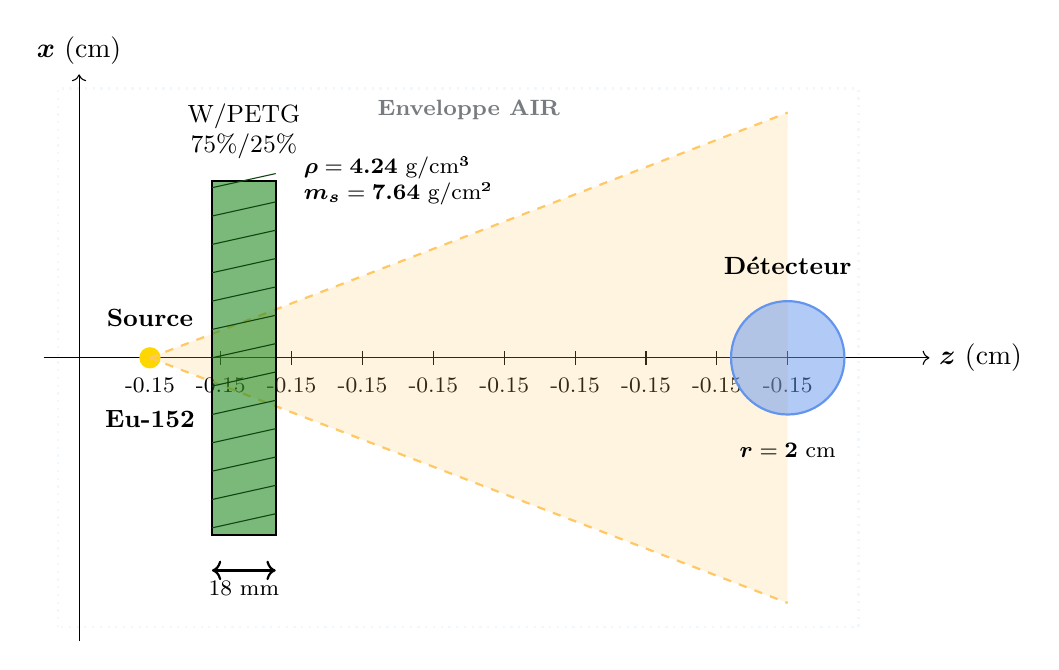
\begin{tikzpicture}[scale=0.9]
    % Cadre et axes
    \draw[->] (-0.5,0) -- (12,0) node[right] {$\bm{z}$ (cm)};
    \draw[->] (0,-4) -- (0,4) node[above] {$\bm{x}$ (cm)};
    
    % Échelle
    \foreach \x in {2,4,6,8,10,12,14,16,18,20} {
        \pgfmathsetmacro{\xpos}{\x/2}
        \draw (\xpos,-0.1) -- (\xpos,0.1);
        \pgfmathparse{int(\x)}
        \node[below,font=\footnotesize] at (\xpos,-0.15) {\pgfmathresult};
    }
    
    % Source (z = 2 cm)
    \fill[source] (1,0) circle (0.15);
    \node[above,font=\small] at (1,0.3) {\textbf{Source}};
    \node[below,font=\small] at (1,-0.6) {\textbf{Eu-152}};
    
    % Cône d'émission (60°)
    \fill[cone,opacity=0.2] (1,0) -- (10,3.46) -- (10,-3.46) -- cycle;
    \draw[cone,thick,dashed] (1,0) -- (10,3.46);
    \draw[cone,thick,dashed] (1,0) -- (10,-3.46);
    
    % Plaque W/PETG pleine (z = 3.75 à 5.55 cm)
    \fill[wpetg,opacity=0.6] (1.875,-2.5) rectangle (2.775,2.5);
    \draw[thick] (1.875,-2.5) rectangle (2.775,2.5);
    
    % Hachures pour W/PETG
    \foreach \y in {-2.4,-2.0,-1.6,-1.2,-0.8,-0.4,0,0.4,0.8,1.2,1.6,2.0,2.4} {
        \draw[wpetg!50!black,thin] (1.875,\y) -- (2.775,\y+0.2);
    }
    
    % Labels plaque
    \draw[<->,thick] (1.875,-3) -- (2.775,-3) node[midway,below,font=\footnotesize] {18 mm};
    \node[font=\small,align=center] at (2.325,3.2) {W/PETG\\75\%/25\%};
    
    % Caractéristiques
    \node[font=\footnotesize,align=left] at (4.5,2.5) {
        $\bm{\rho} = \bm{4.24}$ g/cm³\\
        $\bm{m_s} = \bm{7.64}$ g/cm²
    };
    
    % Détecteur eau (z = 20 cm)
    \fill[water,opacity=0.5] (10,0) circle (0.8);
    \draw[water,thick] (10,0) circle (0.8);
    \node[font=\small] at (10,1.3) {\textbf{Détecteur}};
    \node[font=\footnotesize] at (10,-1.3) {$\bm{r}=\bm{2}$ cm};
    
    % Enveloppe AIR
    \draw[air,thick,dotted] (-0.3,-3.8) rectangle (11,3.8);
    \node[air!50!black,font=\footnotesize] at (5.5,3.5) {\textbf{Enveloppe AIR}};
    
\end{tikzpicture}
\end{figure}

\begin{table}[h!]
\centering
\captionsetup{labelformat=empty}
\caption{\footnotesize Paramètres géométriques des deux configurations}
\begin{tabular}{lcc}
\toprule
\footnotesize \textbf{Paramètre}&\footnotesize \textbf{Bi/PETG (billes)}&\footnotesize \textbf{W/PETG (pleine)}\\
\midrule
\footnotesize Position source $z$&\footnotesize 2.00 cm&\footnotesize 2.00 cm\\
\footnotesize Face avant plaque&\footnotesize 3.75 cm&\footnotesize 3.75 cm\\
\footnotesize Face arrière plaque&\footnotesize 5.55 cm&\footnotesize 5.55 cm\\
\footnotesize Épaisseur totale&\footnotesize 18 mm&\footnotesize 18 mm\\
\footnotesize Position détecteur&\footnotesize 20.00 cm&\footnotesize 20.00 cm\\
\footnotesize Distance source-détecteur&\footnotesize  18 cm&\footnotesize 18 cm\\
\midrule
\footnotesize Dimensions plaque&\footnotesize  $10 \times 10$ cm²&\footnotesize \footnotesize $10 \times 10$ cm²\\
\footnotesize Diamètre billes&\footnotesize  6 mm &\footnotesize  — \\
\footnotesize Nombre de billes&\footnotesize  3402 &\footnotesize  — \\
\bottomrule
\end{tabular}
\end{table}


\newpage

% ============================================================================
% SECTION 2 : ANGLES SOLIDES ET NORMALISATION
% ============================================================================

%==============================================================================
\normalsize
\noindent \begin{mdframed}[backgroundcolor=orange!20]
\section{\Large \color{blue} \textbf{Angles solides et normalisation}\color{black}}
\end{mdframed}
\footnotesize
%==============================================================================

\noindent \begin{mdframed}[backgroundcolor=orange!20]
\subsection{\color{blue}\textbf{Définition des angles solides}\color{black}}
\end{mdframed}
\footnotesize
\medskip

\noindent La source émet des photons dans un cône de demi-angle $\bm{\theta} = \bm{60}°$. L'angle solide correspondant est :

\begin{equation*}
\bm{\Omega_{\text{cône}}} = \bm{2\pi}(\bm{1} - \cos\bm{\theta}) = \bm{\pi}(\bm{1} - \cos \bm{60}°) = \bm{2\pi} \times \bm{0.5} = \bm{\pi} \text{ sr}
\end{equation*}

\noindent La fraction de l'angle solide total ($\bm{4\pi}$ sr) couverte par le cône est :

\begin{equation*}
\bm{f_{\text{cône}}} = \frac{\bm{\Omega_{\text{cône}}}}{\bm{4\pi}} = \frac{\bm{\pi}}{\bm{4\pi}} = \bm{0.25} = \bm{25}\%
\end{equation*}

\noindent \begin{mdframed}[backgroundcolor=orange!20]
\subsection{\color{blue}\textbf{Visualisation du Cône et des Angles Solides}\color{black}}
\end{mdframed}
\footnotesize
\medskip
\begin{figure}[h!]
\centering
\vspace{-0.5cm}
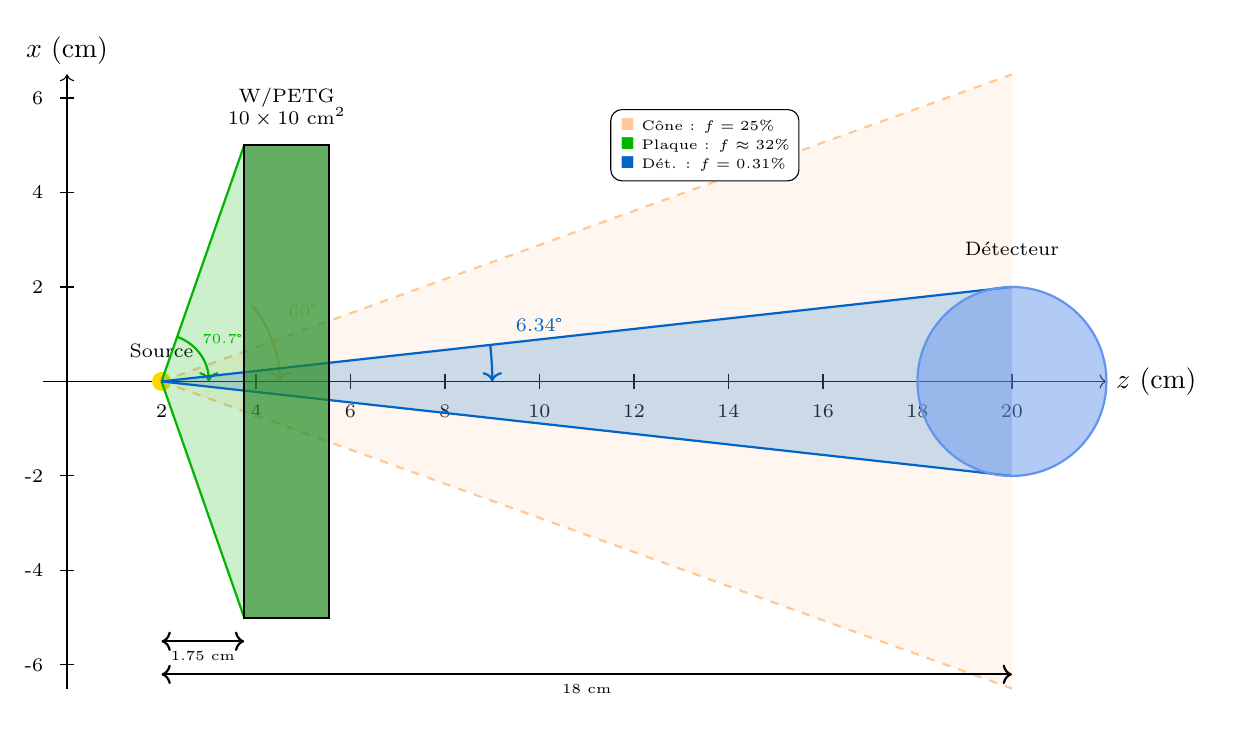
\begin{tikzpicture}[scale=0.6, trim left=-0.5cm]
    
    % AXES - Réduits
    \draw[->] (-0.5,0) -- (22,0) node[right] {$z$ (cm)};
    \draw[->] (0,-6.5) -- (0,6.5) node[above] {$x$ (cm)};  % Réduit de 8 à 6.5
    
    % Échelle sur l'axe z
    \foreach \x in {2,4,6,8,10,12,14,16,18,20} {
        \draw (\x,-0.15) -- (\x,0.15);
        \node[below,font=\scriptsize] at (\x,-0.3) {\x};
    }
    
    % Échelle sur l'axe x - Réduite
    \foreach \y in {-6,-4,-2,2,4,6} {
        \draw (-0.15,\y) -- (0.15,\y);
        \node[left,font=\scriptsize] at (-0.3,\y) {\y};
    }
    
    % SOURCE
    \fill[source] (2,0) circle (0.2);
    \node[above,font=\scriptsize] at (2,0.3) {Source};
    
    % CÔNE D'ÉMISSION 60°
    \fill[cone60,opacity=0.15] (2,0) -- (20,6.5) -- (20,-6.5) -- cycle;
    \draw[cone60,thick,dashed] (2,0) -- (20,6.5);
    \draw[cone60,thick,dashed] (2,0) -- (20,-6.5);
    \draw[cone60,thick,->] (2,0) ++(40:2.5) arc (40:0:2.5);
    \node[cone60,font=\scriptsize] at (5,1.5) {$60$°};
    
    % CÔNE DE LA PLAQUE (vert)
    \fill[coneplaque,opacity=0.2] (2,0) -- (3.75,5) -- (3.75,-5) -- cycle;
    \draw[coneplaque,thick] (2,0) -- (3.75,5);
    \draw[coneplaque,thick] (2,0) -- (3.75,-5);
    \draw[coneplaque,thick,->] (2,0) ++(70:1) arc (70:0:1);
    \node[coneplaque,font=\tiny] at (3.3,0.9) {$70.7$°};
    
    % CÔNE DU DÉTECTEUR (bleu)
    \fill[conedetecteur,opacity=0.2] (2,0) -- (20,2) -- (20,-2) -- cycle;
    \draw[conedetecteur,thick] (2,0) -- (20,2);
    \draw[conedetecteur,thick] (2,0) -- (20,-2);
    \draw[conedetecteur,thick,->] (2,0) ++(6.34:7) arc (6.34:0:7);
    \node[conedetecteur,font=\scriptsize] at (10,1.2) {$6.34$°};
    
    % PLAQUE W/PETG
    \fill[wpetg,opacity=0.7] (3.75,-5) rectangle (5.55,5);
    \draw[black,thick] (3.75,-5) rectangle (5.55,5);
    \node[font=\scriptsize,align=center] at (4.65,5.8) {W/PETG\\$10\times10$ cm$^2$};
    
    % DÉTECTEUR EAU
    \fill[water,opacity=0.5] (20,0) circle (2);
    \draw[water,thick] (20,0) circle (2);
    \node[font=\scriptsize] at (20,2.8) {Détecteur};
    
    % LÉGENDE - Repositionnée
    \node[draw,fill=white,rounded corners,font=\tiny,align=left] at (13.5,5) {%
        \textcolor{cone60}{$\blacksquare$} Cône : $f = 25$\%\\[1pt]
        \textcolor{coneplaque}{$\blacksquare$} Plaque : $f \approx 32$\%\\[1pt]
        \textcolor{conedetecteur}{$\blacksquare$} Dét. : $f = 0.31$\%%
    };
    
    % DISTANCES - Rapprochées
    \draw[<->,thick] (2,-5.5) -- (3.75,-5.5) node[midway,below,font=\tiny] {1.75 cm};
    \draw[<->,thick] (2,-6.2) -- (20,-6.2) node[midway,below,font=\tiny] {18 cm};
    
\end{tikzpicture}%
\vspace{-0.3cm}
\captionsetup{labelformat=empty}
\caption{\footnotesize Comparaison des angles solides : cône d'émission (60°, orange), cône sous-tendu par la plaque (70.7°, vert), et cône du détecteur (6.34°, bleu). La plaque couvre entièrement le cône d'émission.}
\end{figure}

\noindent \begin{mdframed}[backgroundcolor=orange!20]
\subsection{\color{blue}\textbf{Angle Solide de la plaque pleine}\color{black}}
\end{mdframed}
\footnotesize
\medskip

\noindent La plaque carrée de côté $\bm{c} = 10$ cm est située à une distance $\bm{d} = 1.75$ cm de la source (face avant à $\bm{z} = 3.75$ cm, source à $\bm{z} = 2$ cm).

\noindent Le demi-angle $\theta$ sous-tendu par le bord de la plaque est :

\begin{equation*}
\bm{\theta_{\text{plaque}}} = \arctan\left(\frac{\bm{a}}{\bm{d}}\right) = \arctan\left(\frac{\bm{c/2}}{\bm{d}}\right) = \arctan\left(\frac{\bm{5}}{\bm{1.75}}\right) = \arctan(\bm{2.857})
\end{equation*}

\begin{equation*}
\bm{\theta_{\text{plaque}}} = \bm{70.7}°
\end{equation*}

\noindent Pour une surface rectangulaire de dimensions $\bm{2a} \times \bm{2b}$ située à une distance $\bm{d}$ sur l'axe, l'angle solide exact est donné par :

\begin{equation*}
\bm{\Omega} = \bm{4} \arctan\left(\frac{\bm{ab}}{\bm{d}\sqrt{\bm{a^2} + \bm{b^2} + \bm{d^2}}}\right)
\end{equation*}

\noindent Pour une plaque carrée ($\bm{a} = \bm{b} = \bm{5}$ cm) à $\bm{d} = \bm{1.75}$ cm :

\begin{align*}
\bm{\Omega_{\text{plaque}}} &= \bm{4} \arctan\left(\frac{\bm{5} \times \bm{5}}{\bm{1.75} \times \sqrt{\bm{5^2 }+ \bm{5^2} + \bm{1.75^2}}}\right) \\[0.3cm]
&= \bm{4} \arctan\left(\frac{\bm{25}}{\bm{1.75} \times \sqrt{\bm{25} + \bm{25} + \bm{3.06}}}\right) \\[0.3cm]
&= \bm{4} \arctan\left(\frac{\bm{25}}{\bm{1.75} \times \sqrt{\bm{53.06}}}\right) \\[0.3cm]
&= \bm{4} \arctan\left(\frac{\bm{25}}{\bm{1.75} \times \bm{7.28}}\right) \\[0.3cm]
&= \bm{4} \arctan\left(\frac{\bm{25}}{\bm{12.75}}\right) \\[0.3cm]
&= \bm{4} \arctan(\bm{1.961}) \\[0.3cm]
&= \bm{4} \times \bm{1.101} \text{ rad} = \bm{4} \times \bm{63.1}°
\end{align*}

\begin{equation*}
\bm{\Omega_{\text{plaque}}} \approx \bm{4.02} \text{ sr}
\end{equation*}

\noindent La fraction de l'angle solide total ($\bm{4\pi}$ sr) :

\begin{equation*}
\bm{f_{\text{plaque}}} = \frac{\bm{\Omega_{\text{plaque}}}}{\bm{4\pi}} = \frac{\bm{4.02}}{\bm{12.57}} \approx \bm{0.32} = \bm{32}\%
\end{equation*}

\noindent \begin{mdframed}[backgroundcolor=orange!20]
\subsection{\color{blue}\textbf{Angle Solide du Détecteur}\color{black}}
\end{mdframed}
\footnotesize
\medskip

\noindent Le détecteur sphérique de rayon $\bm{r} = \bm{2}$ cm est situé à une distance $\bm{d} = \bm{18}$ cm de la source. Le demi-angle sous-tendu est :

\begin{equation*}
\bm{\theta_{\text{det}}} = \arctan\left(\frac{\bm{r}}{\bm{d}}\right) = \arctan\left(\frac{\bm{2}}{\bm{18}}\right) = \bm{6.34}°
\end{equation*}

\noindent La fraction d'angle solide :

\begin{equation*}
\bm{f_{\text{det}}} = \frac{\bm{1} - \cos(\bm{6.34}°)}{\bm{2}} \approx \bm{0.00306} = \bm{0.306}\%
\end{equation*}

\noindent \begin{mdframed}[backgroundcolor=orange!20]
\subsection{\color{blue}\textbf{Procédure de Normalisation}\color{black}}
\end{mdframed}
\footnotesize
\medskip

\noindent Les formules de normalisation sont :

\begin{align*}
\bm{t_{\text{simulé}}} &= \frac{\bm{N_{\text{events}}}}{\bm{A_{4\pi}}} = \frac{\bm{25} \times \bm{10^6}}{\bm{44000}} = \bm{568.18} \text{ s} \\[0.3cm]
\bm{\dot{D}_{\text{brut}}} &= \frac{\bm{E_{\text{déposée}}}}{\bm{m_{\text{det}}} \times \bm{t_{\text{simulé}}}} \\[0.3cm]
\bm{\dot{D}_{\text{corrigé}}} &= \bm{\dot{D}_{\text{brut}}} \times \bm{f_{\text{cône}}} = \bm{\dot{D}_{\text{brut}}} \times \bm{0.25}
\end{align*}

\newpage

\begin{figure}[h!]
\centering 
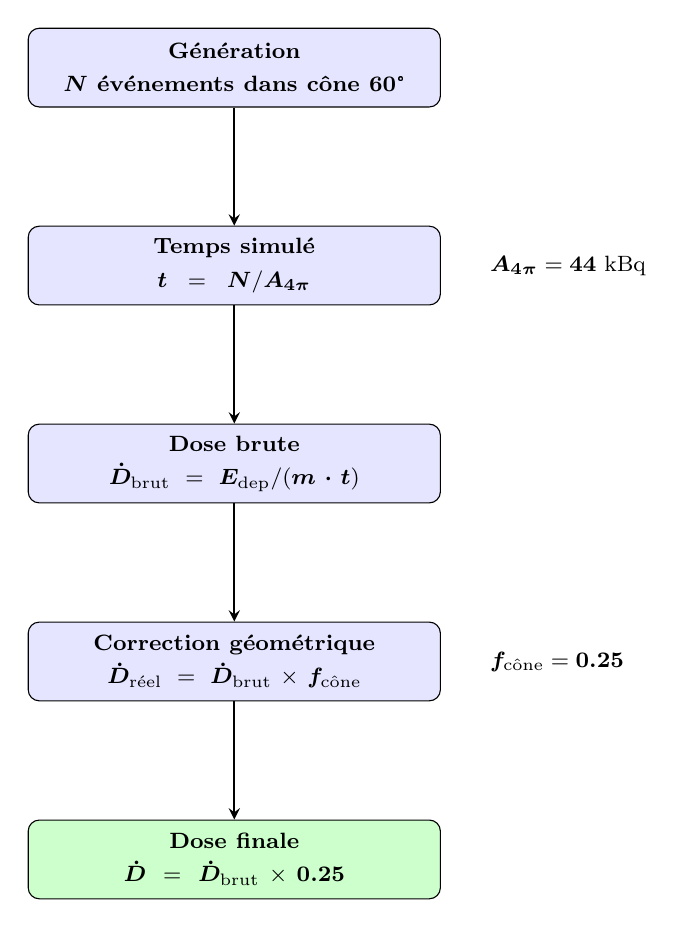
\begin{tikzpicture}[node distance=1.5cm, auto,
    block/.style={rectangle, draw, fill=blue!10, text width=5cm, text centered, rounded corners, minimum height=1cm},
    arrow/.style={thick,->,>=stealth}]
    
    \node[block] (gen) {\footnotesize \textbf{Génération}\\$\footnotesize \bm{N}$  \textbf{événements dans cône 60°}};
    \node[block, below=of gen] (temps) {\footnotesize \textbf{Temps simulé}\\\footnotesize$\bm{t} = \bm{N} / \bm{A_{4\pi}}$};
    \node[block, below=of temps] (dose) {\footnotesize \textbf{Dose brute}\\$\bm{\dot{D}_{\text{brut}}} = \bm{E_{\text{dep}}} / (\bm{m \cdot t})$};
    \node[block, below=of dose] (corr) {\footnotesize \textbf{Correction géométrique}\\\footnotesize $\bm{\dot{D}_{\text{réel}}} = \bm{\dot{D}_{\text{brut}}} \times \bm{f_{\text{cône}}}$};
    \node[block, below=of corr, fill=green!20] (final) {\footnotesize \textbf{Dose finale}\\\footnotesize $\bm{\dot{D}} = \bm{\dot{D}_{\text{brut}}} \times \bm{0.25}$};
    
    \draw[arrow] (gen) -- (temps);
    \draw[arrow] (temps) -- (dose);
    \draw[arrow] (dose) -- (corr);
    \draw[arrow] (corr) -- (final);
    
    % Annotations
    \node[right=0.5cm of temps, font=\small] {\footnotesize $ \bm{A_{4\pi}} = \bm{44}$ kBq};
    \node[right=0.5cm of corr, font=\small] {\footnotesize $\bm{f_{\text{cône}}} = \bm{0.25}$};
    
\end{tikzpicture}
\captionsetup{labelformat=empty}
\caption{\footnotesize Procédure de normalisation pour le calcul du débit de dose.}
\end{figure}


      
%==============================================================================
\normalsize
\noindent \begin{mdframed}[backgroundcolor=orange!20]
\section{\Large \color{blue} \textbf{Bilan des Particules}\color{black}}
\end{mdframed}
\footnotesize
%==============================================================================

\noindent \begin{mdframed}[backgroundcolor=orange!20]
\subsection{\color{blue}\textbf{Statistiques de Génération}\color{black}}
\end{mdframed}
\footnotesize
\medskip

\begin{table}[h!]
\centering
\captionsetup{labelformat=empty}
\caption{\footnotesize Statistiques de génération des gammas (25M événements)}
\begin{tabular}{lrl}
\toprule
\footnotesize \textbf{Paramètre} &\footnotesize  \textbf{Valeur} &\footnotesize  \textbf{Commentaire} \\
\midrule
\footnotesize Événements simulés &\footnotesize  25,000,000 &\footnotesize  — \\
\footnotesize Gammas générés &\footnotesize  48,099,889 &\footnotesize  — \\
\footnotesize Moyenne $\gamma$/événement &\footnotesize  1.924 &\footnotesize  Attendu : 1.924  \\
\footnotesize Événements sans gamma &\footnotesize  $\sim 11\%$ & $P(N=0) \approx 11.7\%$ \\
\midrule
\footnotesize Temps simulé &\footnotesize  568.18 s &\footnotesize  $t = N/A_{4\pi}$ \\
\bottomrule
\end{tabular}
\end{table}

\noindent \begin{mdframed}[backgroundcolor=orange!20]
\subsection{\color{blue}\textbf{Bilan de Transmission}\color{black}}
\end{mdframed}
\footnotesize
\medskip

\begin{table}[h!]
\centering
\captionsetup{labelformat=empty}
\caption{\footnotesize Bilan de transmission à travers la plaque W/PETG}
\begin{tabular}{lrr}
\toprule
\footnotesize \textbf{Catégorie} &\footnotesize  \textbf{Nombre} &\footnotesize  \textbf{Pourcentage} \\
\midrule
\footnotesize Gammas générés (total) &\footnotesize  48,099,889 & 100\% \\
\midrule
\footnotesize Gammas transmis &\footnotesize  8,960,192 &\footnotesize  18.63\% \\
\footnotesize Gammas absorbés &\footnotesize  36,132,636 &\footnotesize  75.12\% \\
\footnotesize Hors acceptance (MISSED) &\footnotesize  $\sim 3,007,061$ &\footnotesize  $\sim 6.25\%$ \\
\midrule
\footnotesize Gammas dans détecteur &\footnotesize  180,750 &\footnotesize  0.376\% \\
\footnotesize Événements avec dépôt &\footnotesize  34,923 &\footnotesize  — \\
\bottomrule
\end{tabular}
\end{table}

\noindent \begin{mdframed}[backgroundcolor=orange!20]
\subsection{\color{blue}\textbf{Visualisation du Bilan Particulaire}\color{black}}
\end{mdframed}
\footnotesize
\medskip

\begin{figure}[h!]
\centering
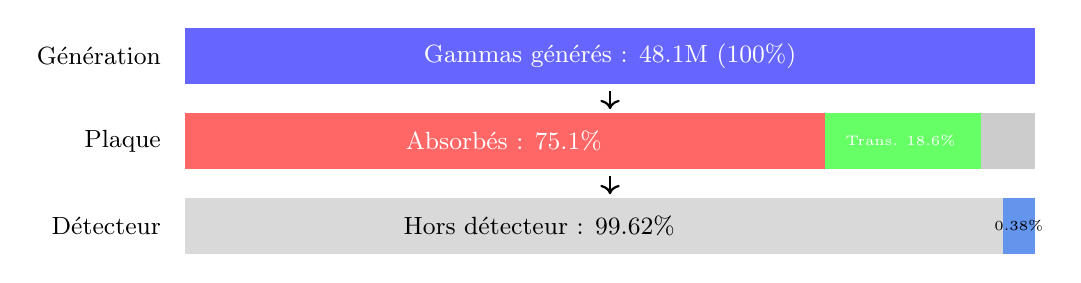
\begin{tikzpicture}[scale=0.9]
    % Barre pour gammas générés
    \fill[blue!60] (0,0) rectangle (12,0.8);
    \node[white,font=\small] at (6,0.4) {Gammas générés : 48.1M (100\%)};
    
    % Barre pour transmission
    \fill[red!60] (0,-1.2) rectangle (9.03,-0.4);
    \node[white,font=\small] at (4.5,-0.8) {Absorbés : 75.1\%};
    
    \fill[green!60] (9.03,-1.2) rectangle (11.24,-0.4);
    \node[white,font=\tiny] at (10.1,-0.8) {Trans. 18.6\%};
    
    \fill[gray!40] (11.24,-1.2) rectangle (12,-0.4);
    
    % Barre pour détecteur
    \fill[gray!30] (0,-2.4) rectangle (11.55,-1.6);
    \fill[water] (11.55,-2.4) rectangle (12,-1.6);
    \node[font=\tiny] at (11.77,-2) {0.38\%};
    \node[font=\small] at (5,-2) {Hors détecteur : 99.62\%};
    
    % Labels
    \node[left,font=\small] at (-0.2,0.4) {Génération};
    \node[left,font=\small] at (-0.2,-0.8) {Plaque};
    \node[left,font=\small] at (-0.2,-2) {Détecteur};
    
    % Flèches
    \draw[->,thick] (6,-0.1) -- (6,-0.35);
    \draw[->,thick] (6,-1.3) -- (6,-1.55);
    
\end{tikzpicture}
\captionsetup{labelformat=empty}
\caption{\footnotesize Bilan des particules : de la génération au détecteur.}
\end{figure}

\newpage

%==============================================================================
\normalsize
\noindent \begin{mdframed}[backgroundcolor=orange!20]
\section{\Large \color{blue} \textbf{Résultats de la simulation du débit de Dose}\color{black}}
\end{mdframed}
\footnotesize
%==============================================================================

\noindent \begin{mdframed}[backgroundcolor=orange!20]
\subsection{\color{blue}\textbf{Méthodes de Calcul}\color{black}}
\end{mdframed}
\footnotesize
\medskip

\noindent Trois méthodes sont utilisées pour calculer le débit de dose :

\begin{enumerate}
    \item \textbf{Méthode 1 (Monte Carlo direct)} : Somme des dépôts d'énergie dans le volume sensible
    \item \textbf{Méthode 1bis (Forçage)} : Estimation du dépôt forcé pour chaque gamma traversant
    \item \textbf{Méthode 2 (Fluence × $\mu_{en}/\rho$)} : Calcul analytique basé sur la fluence
\end{enumerate}

\noindent \begin{mdframed}[backgroundcolor=orange!20]
\subsection{\color{blue}\textbf{Résultats W/PETG Pleine (25M événements)}\color{black}}
\end{mdframed}
\footnotesize
\medskip

\begin{table}[h!]
\centering
\captionsetup{labelformat=empty}
\caption{\footnotesize Résultats de dose pour la configuration W/PETG pleine}
\begin{tabular}{lccc}
\toprule
\textbf{Méthode} & \textbf{Dose (nGy/h)} & \textbf{Incertitude} & \textbf{\% incert.} \\
\midrule
\footnotesize Méthode 1 (MC) &\footnotesize  96.72 &\footnotesize  $\pm 0.68$ &\footnotesize  0.70\% \\
\footnotesize Méthode 1bis (Forçage) &\footnotesize  102.03 &\footnotesize  $\pm 0.24$ & 0.24\% \\
\footnotesize Méthode 2 (Fluence) &\footnotesize  102.03 &\footnotesize  $\pm 0.24$ &\footnotesize  0.24\% \\
\midrule
\footnotesize \textbf{Valeur retenue} &\footnotesize  \color{blue}\textbf{102.0}\color{black} &\footnotesize  $\pm 0.2$ &\footnotesize  0.2\% \\
\bottomrule
\end{tabular}
\end{table}

\end{document}
